
%{{第五十一回}}{第五十一回}}

\chapter{薛小妹新编怀古诗\hspace{.5em}胡庸医乱用虎狼药}

{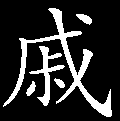
\includegraphics[width=3mm]{../Images/00005}  \kaishu 文有一语写出大景者,如``园中不见一女子''句,俨然大家规模。``疑是姑娘''一语,又俨然庸医口角,新医行径。笔大如椽。}

众人闻得宝琴将素习所经过各省内的古迹为题,作了十首怀古绝句,内隐十物,皆说这自然新巧。都争着看时,只见写道是:

赤壁怀古 其一

赤壁沉埋水不流,徒留名姓载空舟。

喧阗一炬悲风冷,无限英魂在内游。

交趾怀古 其二

铜铸金镛振纪纲,声传海外播戎羌。

马援自是功劳大,铁笛无烦说子房。

钟山怀古 其三

名利何曾伴汝身,无端被诏出凡尘。

牵连大抵难休绝,莫怨他人嘲笑频。

淮阴怀古 其四

壮士须防恶犬欺,三齐位定盖棺时。

寄言世俗休轻鄙,一饭之恩死也知。

广陵怀古 其五

蝉噪鸦栖转眼过,隋堤风景近如何。

只缘占得风流号,惹得纷纷口舌多。

桃叶渡怀古 其六

衰草闲花映浅池,桃枝桃叶总分离。

六朝梁栋多如许,小照空悬壁上题。

青冢怀古 其七

黑水茫茫咽不流,冰弦拨尽曲中愁。

汉家制度诚堪叹,樗栎应惭万古羞。

马嵬怀古 其八

寂寞脂痕渍汗光,温柔一旦付东洋。

只因遗得风流迹,此日衣衾尚有香。

蒲东寺怀古 其九

小红骨贱最身轻,私掖偷携强撮成。

虽被夫人时吊起,已经勾引彼同行。

梅花观怀古 其十

不在梅边在柳边,个中谁拾画婵娟。

团圆莫忆春香到,一别西风又一年。

众人看了,都称奇道妙。宝钗先说道:``前八首都是史鉴上有据的;后二首却无考,我们也不大懂得,不如另作两首为是。''{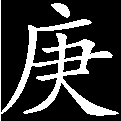
\includegraphics[width=3mm]{../Images/00004}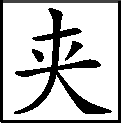
\includegraphics[width=3mm]{../Images/00012}\footnotesize \kaishu 如何?必得宝钗此驳,方是好文。后文若真另作,亦必无趣;若不另作,又有何法省之?看他下文如何。}黛玉忙拦道:{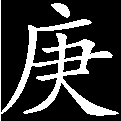
\includegraphics[width=3mm]{../Images/00004}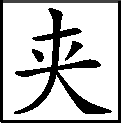
\includegraphics[width=3mm]{../Images/00012}\footnotesize \kaishu 好极!非黛玉不可。脂砚。}``这宝姐姐也忒胶柱鼓瑟、矫揉造作了。这两首虽于史鉴上无考,咱们虽不曾看这些外传,不知底里,难道咱们连两本戏也没有见过不成?那三岁孩子也知道,何况咱们?''探春便道:``这话正是了。''{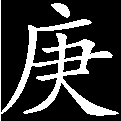
\includegraphics[width=3mm]{../Images/00004}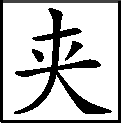
\includegraphics[width=3mm]{../Images/00012}\footnotesize \kaishu 余谓颦儿必有尖语来讽,不望竟有此饰词代为解释,此则真心以待宝钗也。}李纨又道:``况且他原是走到这个地方的。这两件事虽无考,古往今来,以讹传讹,好事者竟故意的弄出这古迹来以愚人。比如那年上京的时节,单是关夫子的坟,倒见了三四处。关夫子一生事业,皆是有据的,如何又有许多的坟?自然是后来人敬爱他生前为人,只怕从这敬爱上穿凿出来,也是有的。及至看《广舆记》上,不止关夫子的坟多,自古来有些名望的,坟就不少,无考的古迹更多。如今这两首虽无考,凡说书唱戏,甚至于求的签上皆有注批,老小男女,俗语口头,人人皆知皆说的。况且又并不是看了《西厢》《牡丹》的词曲,怕看了邪书。这竟无妨,只管留着。''宝钗听说,方罢了。{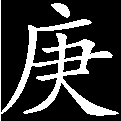
\includegraphics[width=3mm]{../Images/00004}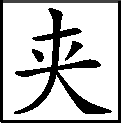
\includegraphics[width=3mm]{../Images/00012}\footnotesize \kaishu 此为三染无痕也,妙极!天衣无缝之文。}大家猜了一回,皆不是。

冬日天短,不觉又是前头吃晚饭之时,一齐前来吃饭。因有人回王夫人说:``袭人的哥哥花自芳进来说,他母亲病重了,想他女儿。他来求恩典,接袭人家去走走。''王夫人听了,便道:``人家母女一场,岂有不许他去的。''一面就叫了凤姐儿来,告诉了凤姐儿,命酌量去办理。

凤姐儿答应了,回至房中,便命周瑞家的去告诉袭人原故。又吩咐周瑞家的:``再将跟着出门的媳妇传一个,你两个人,再带两个小丫头子,跟了袭人去。外头派四个有年纪跟车的。要一辆大车,你们带着坐;要一辆小车,给丫头们坐。''周瑞家的答应了,才要去,凤姐儿又道:``那袭人是个省事的,你告诉说我的话:叫他穿几件颜色好衣裳,大大的包一包袱衣裳拿着,包袱也要好好的,手炉也要拿好的。临走时,叫他先来我瞧瞧。''周瑞家的答应去了。

半日,果见袭人穿戴来了,两个丫头与周瑞家的拿着手炉与衣包。凤姐儿看袭人头上戴着几枝金钗珠钏,倒华丽;又看身上穿着桃红百花刻丝银鼠袄子,葱绿盘金彩绣绵裙,外面穿着青缎灰鼠褂。凤姐儿笑道:``这三件衣裳都是太太的,赏了你倒是好的;但只这褂子太素了些,如今穿着也冷,你该穿一件大毛的。''袭人笑道:``太太就只给了这灰鼠的,还有一件银鼠的。说赶年下再给大毛的,还没有得呢。''凤姐儿笑道:``我倒有一件大毛的,我嫌风毛儿出不好了,正要改去。也罢,先给你穿去罢。等年下太太给作的时节我再作罢,只当你还我一样。''众人都笑道:``奶奶惯会说这话。成年家大手大脚的,替太太不知背地里赔垫了多少东西,真真的赔的是说不出来,那里又和太太算去?偏这会子又说这小气话取笑儿。''凤姐儿笑道:``太太那里想的到这些?究竟这又不是正经事,再不照管,也是大家的体面。说不得我自己吃些亏,把众人打扮体统了,宁可我得个好名也罢了。一个一个像`烧糊了的卷子'似的,人先笑话我当家倒把人弄出个花子来。''众人听了,都叹说:``谁似奶奶这样圣明!在上体贴太太,在下又疼顾下人。''一面说,一面只见凤姐儿命平儿将昨日那件石青刻丝八团天马皮褂子拿出来,与了袭人。又看包袱,只得一个弹墨花绫水红绸里的夹包袱,里面只包着两件半旧棉袄与皮褂。凤姐儿又命平儿把一个玉色绸里的哆啰呢的包袱拿出来,又命包上一件雪褂子。

平儿走去拿了出来,一件是半旧大红猩猩毡的,一件是大红羽纱的。袭人道:``一件就当不起了。''平儿笑道:``你拿这猩猩毡的。把这件顺手拿将出来,叫人给邢大姑娘送去。昨儿那么大雪,人人都是有的,不是猩猩毡就是羽缎羽纱的,十来件大红衣裳,映着大雪好不齐整。就只他穿着那件旧毡斗蓬,越发显的拱肩缩背,好不可怜见的。如今把这件给他罢。''凤姐儿笑道:``我的东西,他私自就要给人。我一个还花不够,再添上你提着,更好了!''众人笑道:``这都是奶奶素日孝敬太太,疼爱下人。若是奶奶素日是小气的,只以东西为事,不顾下人的,姑娘那里还敢这样了。''凤姐儿笑道:``所以知道我的心的,也就是他还知三分罢了。''说着,又嘱咐袭人道:``你妈若好了就罢;若不中用了,只管住下,打发人来回我,我再另打发人给你送铺盖去。可别使人家的铺盖和梳头的家伙。''又吩咐周瑞家的道:``你们自然也知道这里的规矩的,也不用我嘱咐了。''周瑞家的答应:``都知道。我们这去到那里,总叫他们的人回避。若住下,必是另要一两间内房的。''说着,跟了袭人出去,又吩咐预备灯笼,遂坐车往花自芳家来,不在话下。

这里凤姐又将怡红院的嬷嬷唤了两个来,吩咐道:``袭人只怕不来家,你们素日知道那大丫头们,那两个知好歹,派出来在宝玉屋里上夜。你们也好生照管着,别由着宝玉胡闹。''两个嬷嬷去了,一时来回说:``派了晴雯和麝月在屋里,我们四个人原是轮流着带管上夜的。''凤姐儿听了,点头道:``晚上催他早睡,早上催他早起。''老嬷嬷们答应了,自回园去。一时果有周瑞家的带了信回凤姐儿说:``袭人之母业已停床,不能回来。''凤姐儿回明了王夫人,一面着人往大观园去取他的铺盖妆奁。

宝玉看着晴雯麝月二人打点妥当,送去之后,晴雯麝月皆卸罢残妆,脱换过裙袄。晴雯只在熏笼上围坐。麝月笑道:``你今儿别装小姐了,我劝你也动一动儿。''晴雯道:``等你们都去尽了,我再动不迟。有你们一日,我且受用一日。''麝月笑道:``好姐姐,我铺床,你把那穿衣镜的套子放下来,上头的划子划上,你的身量比我高些。''说着,便去与宝玉铺床。晴雯嗐了一声,笑道:``人家才坐暖和了,你就来闹。''此时宝玉正坐着纳闷,想袭人之母不知是死是活,忽听见晴雯如此说,便自己起身出去,放下镜套,划上消息,进来笑道:``你们暖和罢,都完了。''晴雯笑道:``终久暖和不成的,我又想起来汤婆子还没拿来呢。''麝月道:``这难为你想着!他素日又不要汤婆子,咱们那熏笼上暖和,比不得那屋里炕冷,今儿可以不用。''宝玉笑道:``这个话,你们两个都在那上头睡了,我这外边没个人,我怪怕的,一夜也睡不着。''晴雯道:``我是在这里。麝月往他外边睡去。''说话之间,天已二更,麝月早已放下帘幔,移灯炷香,伏侍宝玉卧下,二人方睡。

晴雯自在熏笼上,麝月便在暖阁外边。至三更以后,宝玉睡梦之中,便叫袭人。叫了两声,无人答应,自己醒了,方想起袭人不在家,自己也好笑起来。晴雯已醒,因笑唤麝月道:``连我都醒了,他守在旁边还不知道,真是个挺死尸的。''麝月翻身打个哈气笑道:``他叫袭人,与我什么相干!''因问``作什么?''宝玉说要吃茶,麝月忙起来,单穿红绸小棉袄儿。宝玉道:``披上我的袄儿再去,仔细冷着。''麝月听说,回手便把宝玉披着起夜的一件貂颏满襟暖袄披上,下去向盆内洗手,先倒了一钟温水,拿了大漱盂,宝玉漱了一口;然后才向茶槅上取了茶碗,先用温水涮了一涮,向暖壶中倒了半碗茶,递与宝玉吃了;自己也漱了一漱,吃了半碗。晴雯笑道:``好妹子,也赏我一口儿。''麝月笑道:``越发上脸儿了!''晴雯道:``好妹妹,明儿晚上你别动,我伏侍你一夜,如何?''麝月听说,只得也伏侍他漱了口,倒了半碗茶与他吃过。麝月笑道:``你们两个别睡,说着话儿,我出去走走回来。''晴雯笑道:``外头有个鬼等着你呢。''宝玉道:``外头自然有大月亮的,我们说话,你只管去。''一面说,一面便嗽了两声。

麝月便开了后门,揭起毡帘一看,果然好月色。晴雯等他出去,便欲唬他顽耍。仗着素日比别人气壮,不畏寒冷,也不披衣,只穿着小袄,便蹑手蹑脚的下了熏笼,随后出来。宝玉笑劝道:``看冻着,不是顽的。''晴雯只摆手,随后出了房门。只见月光如水,忽然一阵微风,只觉侵肌透骨,不禁毛骨森然。心下自思道:``怪道人说热身子不可被风吹,这一冷果然利害。''一面正要唬麝月,只听宝玉高声在内道:``晴雯出去了!''晴雯忙回身进来,笑道:``那里就唬死了他?偏你惯会这蝎蝎螫螫老婆汉像的!''宝玉笑道:``倒不为唬坏了他,头一则你冻着也不好;二则他不防,不免一喊,倘或唬醒了别人,不说咱们是顽意,倒反说袭人才去了一夜,你们就见神见鬼的。你来把我的这边被掖一掖。''晴雯听说,便上来掖了掖,伸手进去渥一渥时,宝玉笑道:``好冷手!我说看冻着。''一面又见晴雯两腮如胭脂一般,用手摸了一摸,也觉冰冷。宝玉道:``快进被来渥渥罢。''一语未了,只听咯噔的一声门响,麝月慌慌张张的笑了进来,说道:``吓了我一跳好的。黑影子里,山子石后头,只见一个人蹲着。我才要叫喊,原来是那个大锦鸡,见了人一飞,飞到亮处来,我才看真了。若冒冒失失一嚷,倒闹起人来。''一面说,一面洗手,又笑道:``晴雯出去我怎么不见?一定是要唬我去了。''宝玉笑道:``这不是他,在这里渥呢!我若不叫的快,可是倒唬一跳。''晴雯笑道:``也不用我唬去,这小蹄子已经自怪自惊的了。''一面说,一面仍回自己被中去了。麝月道:``你就这么`跑解马'似的打扮得伶伶俐俐的出去了不成?''宝玉笑道:``可不就这么出去了。''麝月道:``你死不拣好日子!你出去站一站,把皮不冻破了你的。''说着,又将火盆上的铜罩揭起,拿灰锹重将熟炭埋了一埋,拈了两块素香放上,仍旧罩了,至屏后重剔了灯,方才睡下。

晴雯因方才一冷,如今又一暖,不觉打了两个喷嚏。宝玉叹道:``如何?到底伤了风了。''麝月笑道:``他早起就嚷不受用,一日也没吃饭。他这会还不保养些,还要捉弄人。明儿病了,叫他自作自受。''宝玉问:``头上可热?''晴雯嗽了两声,说道:``不相干,那里这么娇嫩起来了。''说着,只听外间房中十锦格上的自鸣钟当当两声,外间值宿的老嬷嬷嗽了两声,因说道:``姑娘们睡罢,明儿再说罢。''宝玉方悄悄的笑道:``咱们别说话了,又惹他们说话。''说着,方大家睡了。

至次日起来,晴雯果觉有些鼻塞声重,懒怠动弹。宝玉道:``快不要声张!太太知道,又叫你搬了家去养息。家去虽好,到底冷些,不如在这里。你就在里间屋里躺着,我叫人请了大夫,悄悄的从后门来瞧瞧就是了。''晴雯道:``虽如此说,你到底要告诉大奶奶一声儿,不然一时大夫来了,人问起来,怎么说呢?''宝玉听了有理,便唤一个老嬷嬷吩咐道:``你回大奶奶去,就说晴雯白冷着了些,不是什么大病。袭人又不在家,他若家去养病,这里更没有人了。传一个大夫,悄悄的从后门进来瞧瞧,别回太太罢了。''老嬷嬷去了半日,来回说:``大奶奶知道了,说两剂药吃好了便罢,若不好时,还是出去为是。如今时气不好,恐沾带了别人事小,姑娘们的身子要紧的。''晴雯睡在暖阁里,只管咳嗽,听了这话,气的喊道:``我那里就害瘟病了,只怕过了人!我离了这里,看你们这一辈子都别头疼脑热的。''说着,便真要起来。宝玉忙按他,笑道:``别生气,这原是他的责任,唯恐太太知道了说他,不过白说一句。你素习好生气,如今肝火自然盛了。''

正说时,人回大夫来了。宝玉便走过来,避在书架之后。只见两三个后门口的老嬷嬷带了一个大夫进来。这里的丫鬟都回避了,有三四个老嬷嬷放下暖阁上的大红绣幔,晴雯从幔中单伸出手去。那大夫见这只手上有两根指甲,足有三寸长,尚有金凤花染的通红的痕迹,便忙回过头来。有一个老嬷嬷忙拿了一块手帕掩了。那大夫方诊了一回脉,起身到外间,向嬷嬷们说道:``小姐的症是外感内滞,近日时气不好,竟算是个小伤寒。幸亏是小姐素日饮食有限,风寒也不大,不过是血气原弱,偶然沾带了些,吃两剂药疏散疏散就好了。''说着,便又随婆子们出去。

彼时,李纨已遣人知会过后门上的人及各处丫鬟回避,那大夫只见了园中的景致,并不曾见一女子。一时出了园门,就在守园门的小厮们的班房内坐了,开了药方。老嬷嬷道:``你老爷且别去,我们小爷罗唆,恐怕还有话说。''大夫忙道:``方才不是小姐,是位爷不成?那屋子竟是绣房一样,又是放下幔子来的,如何是位爷呢?''老嬷嬷悄悄笑道:``我的老爷,怪道小厮们才说今儿请了一位新大夫来了,真不知我们家的事。那屋子是我们小哥儿的,那人是他屋里的丫头,倒是个大姐,那里的小姐?若是小姐的绣房,小姐病了,你那么容易就进去了?''说着,拿了药方进去。

宝玉看时,上面有紫苏、桔梗、防风、荆芥等药,后面又有枳实、麻黄。宝玉道:``该死,该死,他拿着女孩儿们也像我们一样的治,如何使得!凭他有什么内滞,这枳实、麻黄如何禁得。谁请了来的?快打发他去罢!再请一个熟的来。''老婆子道:``用药好不好,我们不知道这理。如今再叫小厮去请王太医去倒容易,只是这大夫又不是告诉总管房请来的,这轿马钱是要给他的。''宝玉道:``给他多少?''婆子道:``少了不好看,也得一两银子,才是我们这门户的礼。''宝玉道:``王太医来了给他多少?''婆子笑道:``王太医和张太医每常来了,也并没个给钱的,不过每年四节大趸送礼,那是一定的年例。这人新来了一次,须得给他一两银子去。''宝玉听说,便命麝月去取银子。麝月道:``花大奶奶还不知搁在那里呢?''宝玉道:``我常见他在螺甸小柜子里取钱,我和你找去。''说着,二人来至宝玉堆东西的房子,开了螺甸柜子,上一格子都是些笔墨、扇子、香饼、各色荷包、汗巾等物;下一格却是几串钱。于是开了抽屉,才看见一个小簸箩内放着几块银子,倒也有一把戥子。麝月便拿了一块银子,提起戥子来问宝玉:``那是一两的星儿?''宝玉笑道:``你问我?有趣,你倒成了才来的了。''麝月也笑了,又要去问人。宝玉道:``拣那大的给他一块就是了。又不作买卖,算这些做什么!''麝月听了,便放下戥子,拣了一块掂了一掂,笑道:``这一块只怕是一两了。宁可多些好,别少了,叫那穷小子笑话,不说咱们不识戥子,倒说咱们有心小器似的。''那婆子站在外头台矶上,笑道:``那是五两的锭子夹了半边,这一块至少还有二两呢!这会子又没夹剪,姑娘收了这块,再拣一块小些的罢。''麝月早掩了柜子出来,笑道:``谁又找去!多了些你拿了去罢。''宝玉道:``你只快叫茗烟再请王大夫去就是了。''婆子接了银子,自去料理。

一时茗烟果请了王太医来,诊了脉后,说的病症与前相仿,只是方上果没有枳实、麻黄等药,倒有当归、陈皮、白芍等,药之分量较先也减了些。宝玉喜道:``这才是女孩儿们的药,虽然疏散,也不可太过。旧年我病了,却是伤寒内里饮食停滞,他瞧了,还说我禁不起麻黄、石膏、枳实等狼虎药。我和你们一比,我就如那野坟圈子里长的几十年的一棵老杨树,你们就如秋天芸儿进我的那才开的白海棠,连我禁不起的药,你们如何禁得起。''麝月等笑道:``野坟里只有杨树不成?难道就没有松柏?我最嫌的是杨树,那么大笨树,叶子只一点子,没一丝风,他也是乱响。你偏比他,也太下流了。''宝玉笑道:``松柏不敢比。连孔子都说:`岁寒然后知松柏之后凋也。'可知这两件东西高雅,不怕羞臊的才拿他混比呢。''

说着,只见老婆子取了药来。宝玉命把煎药的银吊子找了出来,{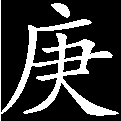
\includegraphics[width=3mm]{../Images/00004}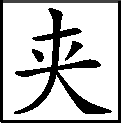
\includegraphics[width=3mm]{../Images/00012}\footnotesize \kaishu ``找''字神理,乃不常用之物也。}就命在火盆上煎。晴雯因说:``正经给他们茶房里煎去,弄得这屋里药气,如何使得。''宝玉道:``药气比一切的花香果子香都雅。神仙采药烧药,再者高人逸士采药治药,最妙的一件东西。这屋里我正想各色都齐了,就只少药香,如今恰好全了。''一面说,一面早命人煨上。又嘱咐麝月打点东西,遣老嬷嬷去看袭人,劝他少哭。一一妥当,方过前边来贾母王夫人处问安吃饭。

正值凤姐儿和贾母王夫人商议说:``天又短又冷,不如以后大嫂子带着姑娘们在园子里吃饭一样。等天长暖和了,再来回的跑也不妨。''王夫人笑道:``这也是好主意。刮风下雪倒便宜。吃些东西受了冷气也不好;空心走来,一肚子冷风,压上些东西也不好。不如后园门里头的五间大房子,横竖有女人们上夜的,挑两个厨子女人在那里,单给他姊妹们弄饭。新鲜菜蔬是有分例的,在总管房里支去,或要钱,或要东西;那些野鸡、獐、狍各样野味,分些给他们就是了。''贾母道:``我也正想着呢,就怕又添一个厨房多事些。''凤姐道:``并不多事。一样的分例,这里添了,那里减了。就便多费些事,小姑娘们冷风朔气的,{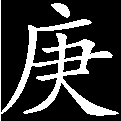
\includegraphics[width=3mm]{../Images/00004}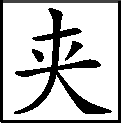
\includegraphics[width=3mm]{../Images/00012}\footnotesize \kaishu ``朔''字又妙!``朔''作``韶'',北音也。用北音,奇想奇想。}别人还可,第一林妹妹如何禁得住?就连宝兄弟也禁不住,何况众位姑娘。''贾母道:``正是这话了。上次我要说这话,我见你们的大事太多了,如今又添出这些事来,\ldots{}\ldots{}''要知端的------

{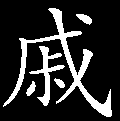
\includegraphics[width=3mm]{../Images/00005}  \kaishu 总评:此回再从猜谜着色,便与前回重复,且又是一幅即景联诗图矣,成何趣味?就灯谜中生一番讥评,别有清思,迥非凡艳。}

{搁起灯谜,接入袭人了,却不就袭人一面写照,作者大有苦心。盖袭人不盛饰,则非大家威仪,如盛饰,又岂有其母临危而盛饰者乎?在凤姐一面,于衣服车马仆从房屋铺盖等物一一检点,色色亲嘱,既得掌家人体统,而袭人之俊俏风神毕现。}

{文有数千言写一琐事者,如一吃茶,偏能于未吃以前、既吃以后,细细描写;如一拿银,偏能于开柜时生无数波折,{{(平)}}{[}秤{]}银时又生无数波折。心细如发。}
